\section{Luồng upload/run model}

Luồng này mô tả quy trình đưa một mô hình Rasa mới vào hệ thống và kích hoạt mô hình đó để phục vụ chatbot. Đây là luồng quản trị vận hành, thường được sử dụng khi đã có mô hình huấn luyện sẵn và cần cập nhật môi trường chạy mà không phải sửa trực tiếp trong mã nguồn ứng dụng.

\begin{figure}[H]
    \centering
    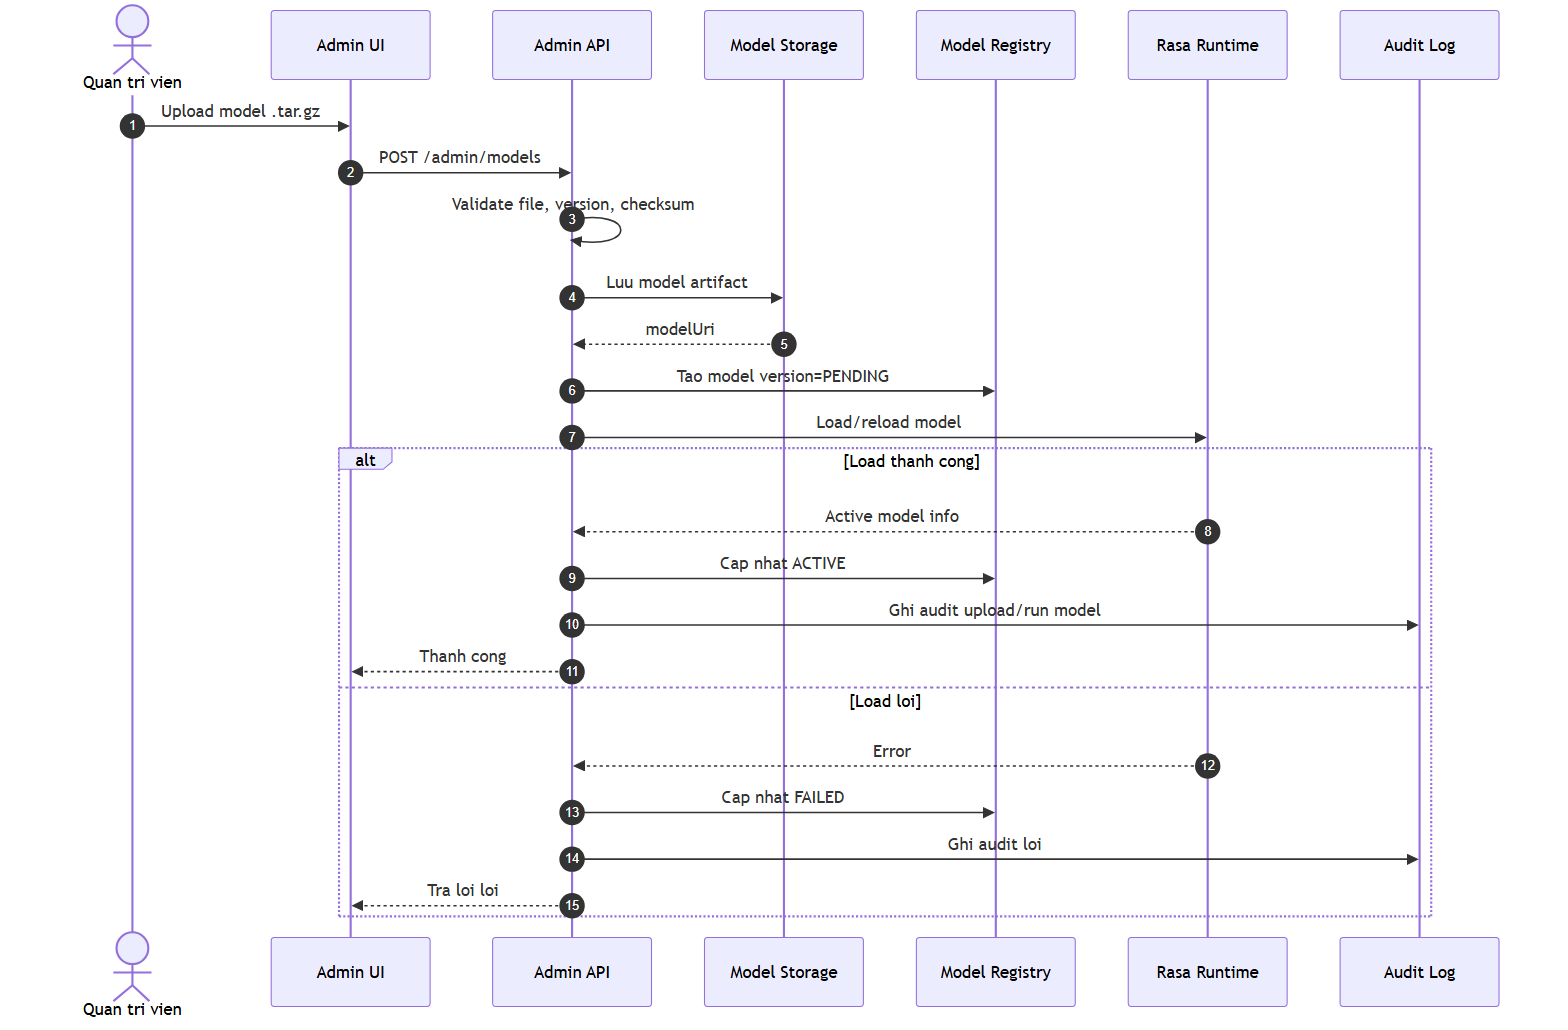
\includegraphics[width=\textwidth]{content/source/mermaid_sequence/seq_03.png}
    \caption{Luồng upload/run model}
\end{figure}

Theo sequence, người quản trị chọn mô hình hoặc gói mô hình trên giao diện, frontend tải tệp lên backend quản trị, sau đó backend lưu mô hình, cập nhật metadata và yêu cầu Rasa nạp mô hình tương ứng. Sau khi thao tác hoàn tất, trạng thái mô hình đang chạy được phản hồi trở lại để giao diện hiển thị kết quả. Luồng này tách riêng bước quản lý tệp mô hình và bước kích hoạt runtime, nhờ đó hệ thống có thể kiểm soát lịch sử mô hình tốt hơn.
